\section{Decomposition view (UML Component diagram)}\label{sec:decomposition}
In this section, we decompose our system to the necessary level of detail. The subsystems are each decomposed as necessary to provide a clear view on the system, and components are added and explained according to the non-functional requirements, where applicable. Each decomposition is accompanied by a detailed diagram for reference.

\subsection{CommunicationSubsystem}
\begin{figure}[!htp]
    \centering
    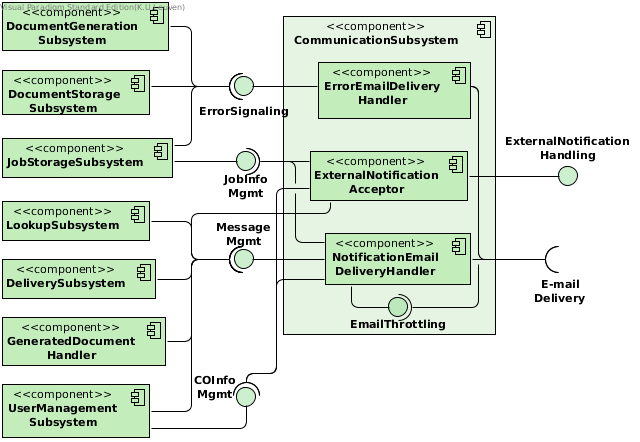
\includegraphics[width=0.7\textwidth]{figures/Communication Subsystem.png}
    \caption{Decomposition of \texttt{CommunicationSubsystem}}\label{fig:decomp-commsub}
\end{figure}

The \ttt{CommunicationSubsystem} is decomposed conform figure \ref{fig:decomp-commsub}. For notification of the eDocs administrators according to requirements \emph{Av1a}, \emph{Av2a} and \emph{Av3}, we split the communication subsystem into a standard communication module, the \ttt{NotificationEmailDeliveryHandler}, and onde dedicated to notify the eDocs administrators, namely the \ttt{ErrorEmailDeliveryHandler}. The latter can throttle the workings of the former, so it has precedence in e-mail communication out of the system. This allows us to guarantee an optimal notification time. The semantical difference between the message handlers being that the \ttt{ErrorEmailDeliveryHandler} handles errors internal to the system, while the \ttt{NotificationEmailDeliveryHandler} handles standard notification, document delivery emails, errors introduced externally to the system e.g. raw data errors etc. Functionally, we introduced another component, the \ttt{ExternalNotificationAcceptor}, which accepts external messages to the system e.g. receipt tracking notifications from zoomit or e-mail delivery failure notifications. The component thus allows external messages to be accepted or rerouted (e.g. to a Customer Administrator) by the system.

\subsection{DeliverySubsystem}
\begin{figure}[!htp]
    \centering
    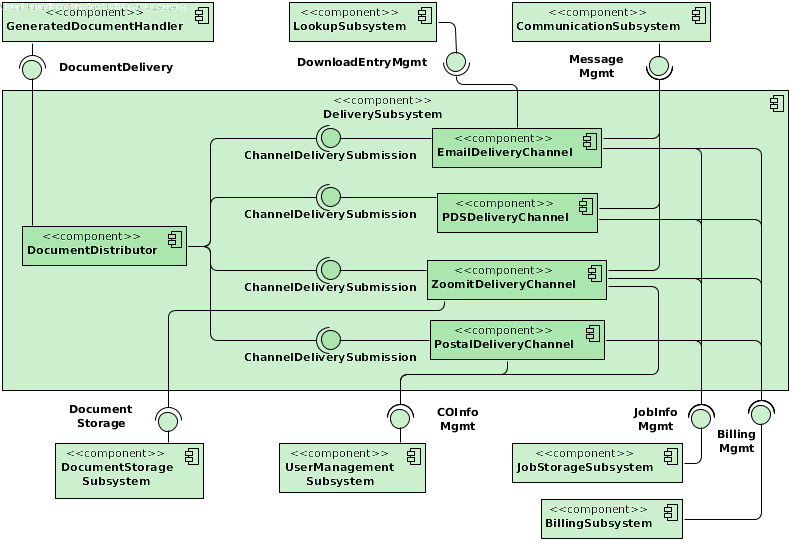
\includegraphics[width=0.9\textwidth]{figures/Delivery Subsystem.png}
    \caption{Decomposition of \texttt{DeliverySubsystem}}\label{fig:decomp-delisub}
\end{figure}

The \ttt{DeliverySubsystem} is decomposed conform figure \ref{fig:decomp-delisub}. For requirements \emph{M2}, \emph{M3} concerning print \& postal service delivery and \emph{Av3} concerning zoomit delivery, we split the different delivery methods into dedicated components, called \ttt{DeliveryChannel}s. These are governed by a \ttt{DocumentDistributor} to keep the \ttt{Channels} separate from each other and the rest of the system. This use of \emph{Hiding Information}, \emph{Abstract common services} and \emph{Using an intermediary} allows us to conform to \emph{M2} and \emph{M3}. The \ttt{ZoomitDeliveryChannel} will be further decomposed in section \ref{sec:decomp-zoomitchan}, for \emph{Av3}.

\subsection{ZoomitDeliveryChannel}\label{sec:decomp-zoomitchan}
\begin{figure}[!htp]
    \centering
    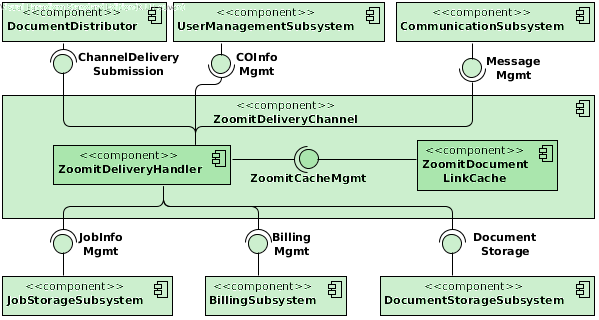
\includegraphics[width=0.6\textwidth]{figures/ZoomitDeliveryChannel.png}
    \caption{Decomposition of \texttt{ZoomitDeliveryChannel}}\label{fig:decomp-zoomitchan}
\end{figure}

The \ttt{ZoomitDeliveryChannel} is decomposed conform figure \ref{fig:decomp-zoomitchan}. We introduced a \ttt{ZoomitDocumentLinkCache} for \emph{Av3}, which states that up to two days of undelivered documents should be cached by the system. This cache keeps the \ttt{JobID} and \ttt{DeliveryMetaData} corresponding to documents that could not be delivered. The other component, the \ttt{ZoomitDeliveryHandler}, takes care of all the rest of Zoomit delivery, and checks and decides when the cache has to be used (when the service is down). The \ttt{ZoomitDeliveryHandler} will take care of the exponential backoff and retries, and notify the eDocs Administrator as stated in \emph{Av3}.

\subsection{DocumentGenerationSubsystem}
\begin{figure}[!htp]
    \centering
    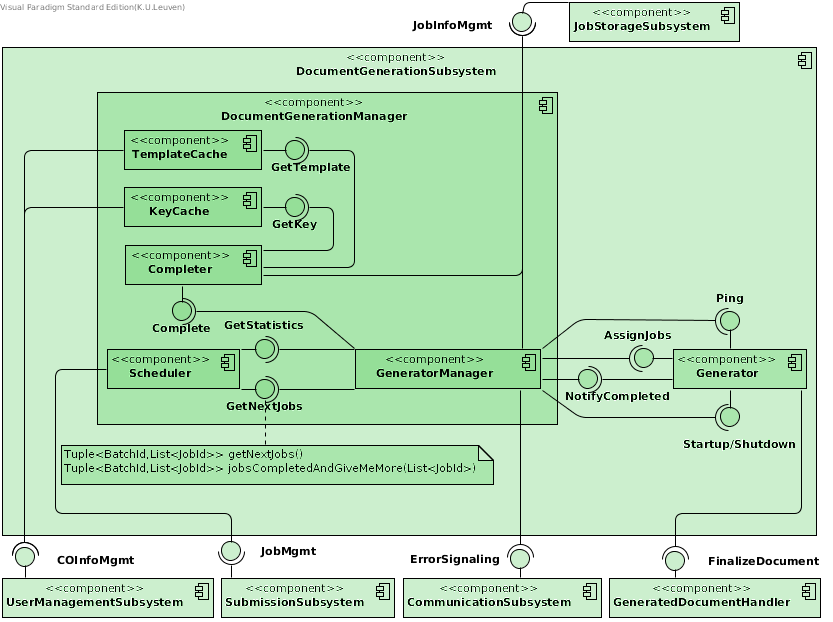
\includegraphics[width=0.9\textwidth]{figures/Document Generation Subsystem.png}
    \caption{Decomposition of \texttt{DocumentGenerationSubsystem}}\label{fig:decomp-docgensub}
\end{figure}

The \ttt{DocumentGenerationSubsystem} is decomposed conform figure \ref{fig:decomp-docgensub}. This has remained largely the same as at the beginning of the assingment, with some modification to the interfaces after decomposition.

\subsection{DocumentStorageSubsystem}\label{sec:decomp-docstosub}
\begin{figure}[!htp]
    \centering
    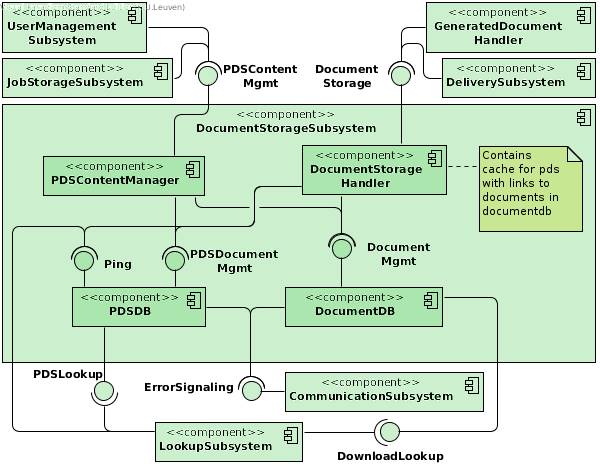
\includegraphics[width=0.6\textwidth]{figures/Document Storage Subsystem.png}
    \caption{Decomposition of \texttt{DocumentStorageSubsystem}}\label{fig:decomp-docstosub}
\end{figure}

The \ttt{DocumentStorageSubsystem} is decomposed conform figure \ref{fig:decomp-docstosub}. We introduced separate \ttt{PDSDB} and \ttt{DocumentDB} components for \emph{Av2}. The requirement demands that when the storage for the PDS fails, the rest of the system is not impacted. If we do not include a general \ttt{DocumentDB} for storing all documents (including the ones ``replicated'' in the \ttt{PDSDB}), this guarantee cannot be made. \emph{P2} also warrants this division, by making lookups of download documents and PDS document have little to no impact on eachother performancewise. They are both governed by the \ttt{DocumentStorageHandler}, which signals the databases to store documents where necessary, handles filling of the \ttt{PDSDB} when a Recipient registers, and has caching functionality for \ttt{Av2}. For more information regarding the \ttt{DocumentStorageHandler}, see section \ref{sec:decomp-docstohan}.

\subsection{DocumentStorageHandler}\label{sec:decomp-docstohan}
\begin{figure}[!htp]
    \centering
    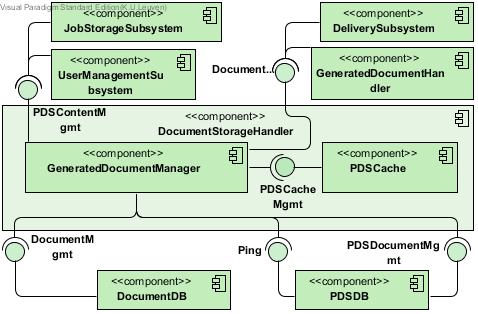
\includegraphics[width=0.6\textwidth]{figures/DocumentStorageHandler.png}
    \caption{Decomposition of \texttt{DocumentStorageHandler}}\label{fig:decomp-docstohan}
\end{figure}

The \ttt{DocumentStorageHandler} is decomposed conform figure \ref{fig:decomp-docstohan}. Next to the \ttt{GeneratedDocumentManager}, which has all general functionality of the \ttt{DocumentStorageHandler}, we introduce a \ttt{PDSCache} for \emph{Av2}. The goal of this cache is to store IDs of documents with the \ttt{PDSDB} as destination, when the \ttt{PDSDB} fails. This can be both in the case when a newly generated document arrives as when a Recipient registers and his document have to be added to the \ttt{PDSDB} from the \ttt{DocumentDB} (an action also performed by the \ttt{GeneratedDocumentManager}).

\subsection{DocumentDB}
\begin{figure}[!htp]
    \centering
    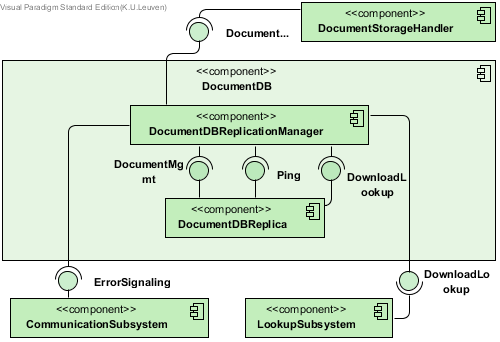
\includegraphics[width=0.6\textwidth]{figures/DocumentDB.png}
    \caption{Decomposition of \texttt{DocumentDB}}\label{fig:decomp-docdb}
\end{figure}

The \ttt{DocumentDB} is decomposed conform figure \ref{fig:decomp-docdb}. We have introduced \emph{Active replication} to the general \ttt{DocumentDB} with a \ttt{DocumentDBReplicationManager} and multiple \ttt{DocumentDBReplica}s, for various reasons. A first and simple reason is architectural consistency with the \ttt{PDSDB}, but more importantly are reasons pertaining \emph{Av2}: When caching a document for the PDS, a link to the document in the \ttt{DocumentDB} is stored in the cache. This warrants replication in the \ttt{DocumentDB} because, while the \ttt{DocumentDB} seems an innocent bystander, its failure would obstruct the caching of documents. \emph{P2} also warrants this introduction, because it makes the sharding of the replicas possible. A system to form shards of replicas would allow the \ttt{DocumentDBReplicationManager} to select a shard not currently under load to answer a lookup request directly to a user session, thus allowing for better performance. We have not opted for an additional division in short and long term since this database is always under heavy use, and this additional functionality would place more load on the replicas.

\subsection{PDSDB}
\begin{figure}[!htp]
    \centering
    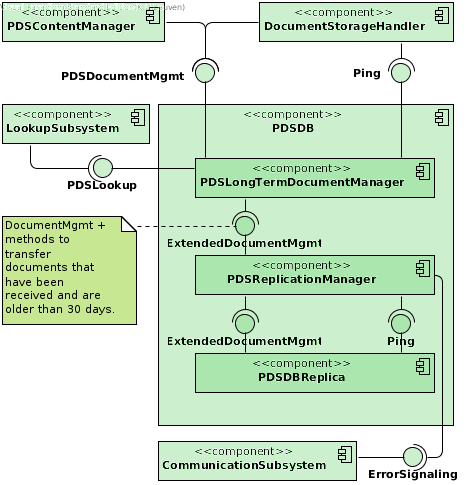
\includegraphics[width=0.5\textwidth]{figures/PDSDB.png}
    \caption{Decomposition of \texttt{PDSDB}}\label{fig:decomp-pdsdb}
\end{figure}

The \ttt{PDSDB} is decomposed conform figure \ref{fig:decomp-pdsdb}. This has remained largely the same as at the beginning of the assingment, with some modification to the interfaces after decomposition. We have added a \ttt{Ping} interface to the \ttt{PDSLongTermDocumentManager}, so the \ttt{DocumentStorageHandler} can check whether the whole \ttt{PDSDB} has failed, for caching reasons (\emph{Av2}).

\subsection{JobStorageSubsystem}
\begin{figure}[!htp]
    \centering
    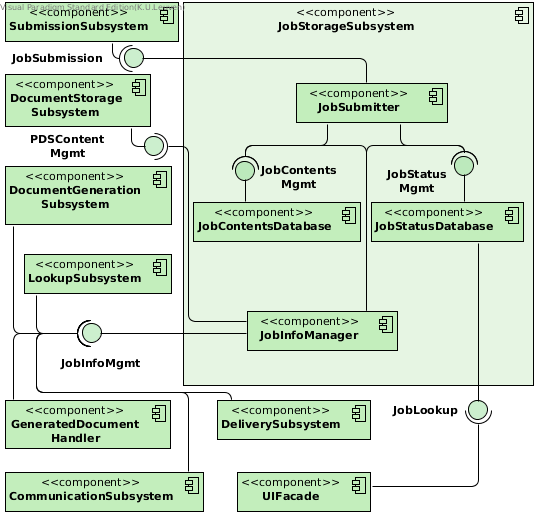
\includegraphics[width=0.6\textwidth]{figures/Job Storage Subsystem.png}
    \caption{Decomposition of \texttt{JobStorageSubsystem}}\label{fig:decomp-jobsub}
\end{figure}

The \ttt{JobStorageSubsystem} is decomposed conform figure \ref{fig:decomp-jobsub}. We have introduced two databases: the \ttt{JobStatusDatabase} and the \ttt{JobContentsDatabase}. The former stores only the statuses of jobs, which is important for \emph{P2}, while the latter stores everything else. A dedicated database for the statuses, which can be directly queried, allows the system to satisfy \emph{P2}. We have introduced two managing components for these database: the \ttt{JobSubmitter} and the \ttt{JobInfoManager}. The \ttt{JobSubmitter} submits new jobs from the submission subsystem. It creates entries in both databases, but only once per job. The \ttt{JobInfoManager} can be contacted by the rest of the system to update entries in both databases, e.g. update the status of a job to ``Temporarily failed'', or signal the \ttt{JobContentsDatabase} it can remove the plain \ttt{RawData} from an entry (whilst keeping the delivery data etc.). The division of these components forms a small advantage, not only in coherence, but for \emph{P2} as well: balancing submission and update load between these components keeps the status database optimally up-to-date (consistent in time).

\subsection{LookupSubsystem}
\begin{figure}[!htp]
    \centering
    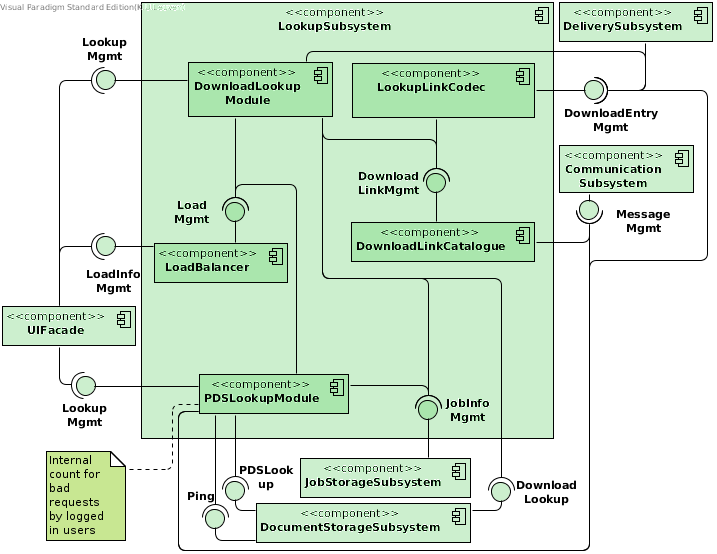
\includegraphics[width=0.75\textwidth]{figures/Lookup Subsystem.png}
    \caption{Decomposition of \texttt{LookupSubsystem}}\label{fig:decomp-lookupsub}
\end{figure}

The \ttt{LookupSubsystem} is decomposed conform figure \ref{fig:decomp-lookupsub}. This decomposition is warranted by \emph{P2}. The lookup functionality is decomposed into a \ttt{DownloadLookupModule}, a \ttt{PDSLookupModule} and a \ttt{LoadBalancer} with behaviour as described in \ref{march:p2} pertaining load balancing. A \ttt{LookupLinkCodec} has been introduced for fast and modular encoding and decoding of Document IDs into links for lookups. This is complemented with a \ttt{DownloadLinkCatalogue} internal to the \ttt{Subsystem}, where the validity of a download lookup request can be verified immediately. This is the source of a performance gain since it doesn't have to happen deeper in the system, e.g. after already looking up the document or contacting other subsystems. The \ttt{DownloadLinkCatalogue} thus keeps track of expiration of download link itself.

\subsection{SubmissionSubsystem}
\begin{figure}[!htp]
    \centering
    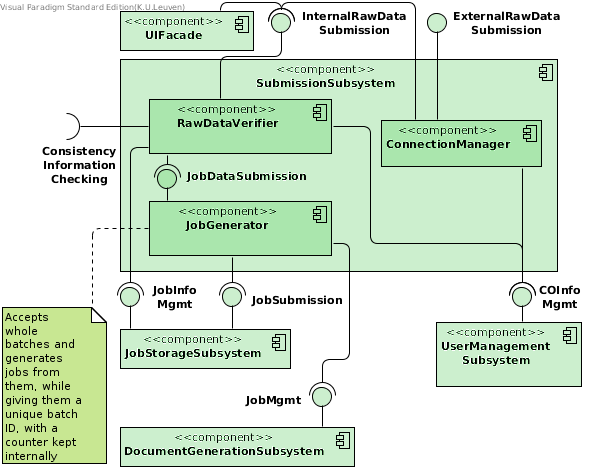
\includegraphics[width=0.75\textwidth]{figures/Submission Subsystem.png}
    \caption{Decomposition of \texttt{SubmissionSubsystem}}\label{fig:decomp-submsub}
\end{figure}

The \ttt{SubmissionSubsystem} is decomposed conform figure \ref{fig:decomp-submsub}. This decomposition is mainly based on functional needs, and for clarification of behaviour of \emph{UC3}. The \ttt{ConnectionManager} manages external submission of raw data conform protocols offered by the system. The \ttt{RawDataVerifier} accepts Raw Data Batches from the \ttt{ConnectionManager} or the \ttt{UIFacade} (internal submission by a Customer Administrator), and verifies the content. The \ttt{JobGenerator} then creates jobs from the Raw Data batches and submits them to both the \ttt{JobStorageSubsystem} and the \ttt{DocumentGenerationSubsystem}.

\subsection{UIFacade}
\begin{figure}[!htp]
    \centering
    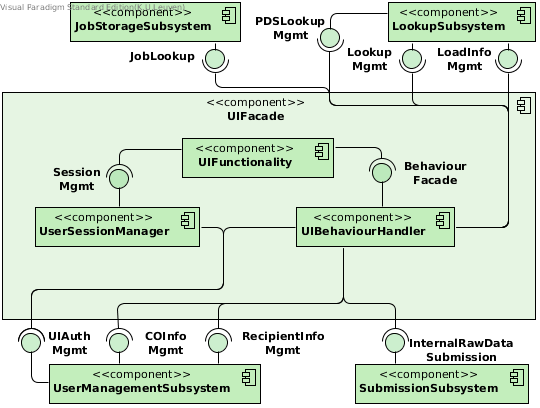
\includegraphics[width=0.6\textwidth]{figures/UI Facade.png}
    \caption{Decomposition of \texttt{UIFacade}}\label{fig:decomp-uif}
\end{figure}

The \ttt{UIFacade} is decomposed conform figure \ref{fig:decomp-uif}. This decomposition slightly supports \emph{P2} by supplying the user session infrastructure as used by the shards of the \ttt{DocumentDB}. The \ttt{UIBehaviourHandler} handles the rest of the \ttt{UIFacade}'s functionality.

\subsection{UserManagementSubsystem}\label{sec:decomp-usersub}
\begin{figure}[!htp]
    \centering
    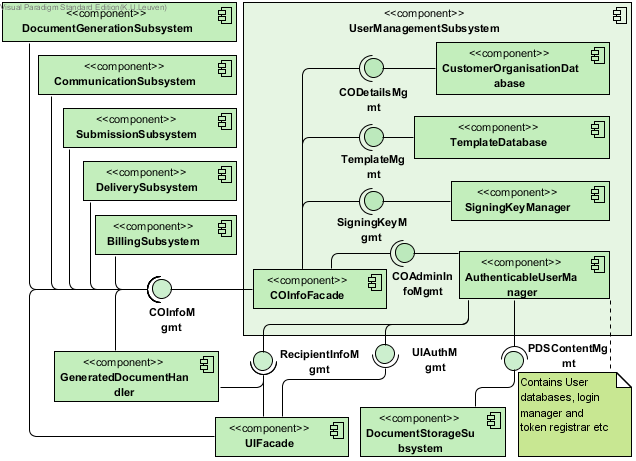
\includegraphics[width=0.7\textwidth]{figures/User Managment Subsystem.png}
    \caption{Decomposition of \texttt{UserManagementSubsystem}}\label{fig:decomp-usersub}
\end{figure}

The \ttt{UserManagementSubsystem} is decomposed conform figure \ref{fig:decomp-usersub}. The main driver for this decomposition is \emph{M1}. For this requirement, we introduced th \ttt{TemplateDatabase}, where part of the modifications for the requirement are confined and protected from the rest of the system. We then added the other databases, splitting them up where logical, and added a facade under the form of the \ttt{COInfoFacade} for most of the Customer Organization Information lookups. The other databases are slightly detailed and not warranted by the requirement, but they are also added for functional behaviour and clearer scenarios.

\subsection{AuthenticableUserManager}
\begin{figure}[!htp]
    \centering
    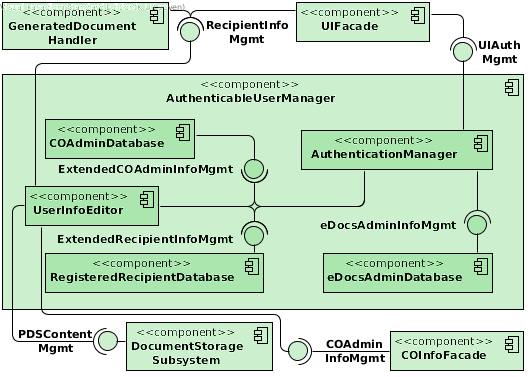
\includegraphics[width=0.6\textwidth]{figures/AuthenticableUserManager.png}
    \caption{Decomposition of \texttt{AuthenticableUserManager}}\label{fig:decomp-authuserman}
\end{figure}

The \ttt{AuthenticableUserManager} is decomposed conform figure \ref{fig:decomp-authuserman}. This is one of the databases introduced in decomposition \ref{sec:decomp-usersub}. It is as mentioned also mainly decomposed for functional behaviour and clearer scenarios, without extended demand of a non-functional requirement.

\begin{comment}
\subsection{BillingSubsystem}
\begin{figure}[!htp]
    \centering
    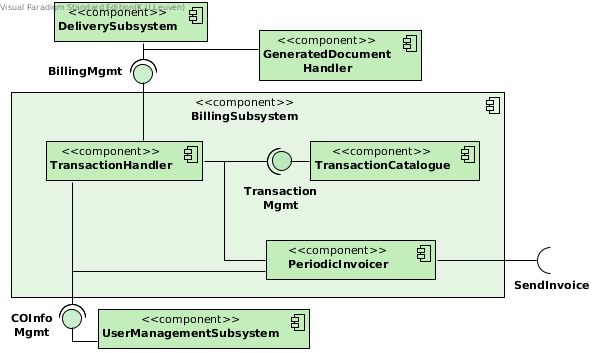
\includegraphics[width=\textwidth]{figures/Billing Subsystem.png}
    \caption{Decomposition of \texttt{BillingSubsystem}}\label{fig:decomp-billingsub}
\end{figure}

The \ttt{} is decomposed conform figure \ref{fig:decomp-}.
\end{comment}